\section{Mathematical Formulation}
\label{sec:mathematical}
To study the spread of news in the population, three types of agents are considered: individuals (also called "people"), \textit{real} news sources, and \textit{fake} news sources. In the context of this research, we define a real news source as a source which does its best effort to spread reliable, unbiased and fact-checked information. Its opposite, the fake news source, has interest in spreading false information and actively and purposely does it. An example of one such network can be seen in Figure~\ref{pics:network_example}.

\begin{figure}
\centering
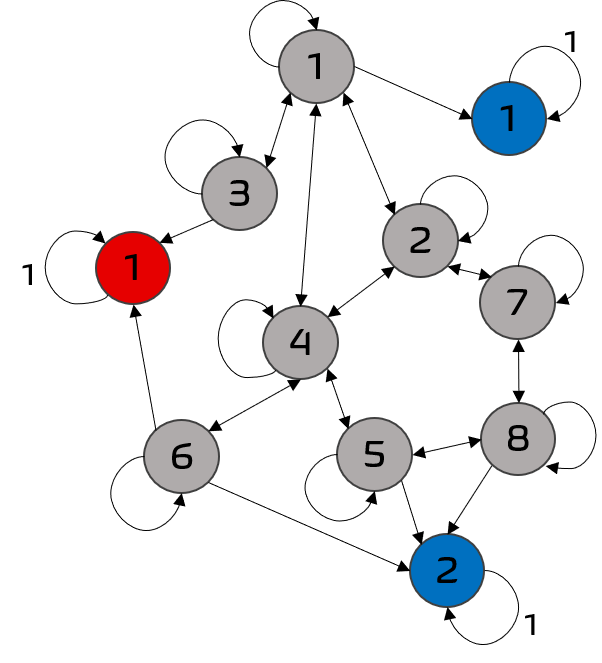
\includegraphics[width=2.5in]{Figures/network_example.png}
\caption{Example of one network that could be generated with our model. The directed graph is formed by eight individuals 1-8, one source of fake news (red), two sources of real news (blue), and links between nodes. Every node has a self loop, with weight 1 for the news sources, and the news sources only have in-neighbors.}
\label{pics:network_example}
\end{figure}
In order to be able to use a multitude of theoretical and analytical tools learned during the course, a linear model with the following update equation is studied
\begin{equation}
\label{eq:model}
x(k+1) = A x(k),
\end{equation}
where $x_i(k) \in [-1;1]$ represents the opinion of individual or source  $i$ at timestep $k$ and $A$ is the adjacency matrix of the network, as in the popular opinion model\cite{Friedkin1990}.
Constructing the adjacency matrix $A$ is a non-trivial task as it requires several assumptions on the the existence of links between people, the existence of links between people and news sources, and the importance of each such link.
The existence of links between different individuals and between individuals and sources is determined either by their physical distance or randomly, as will be explained in more detail in Subsection~\ref{subsec:connections_existence}.
To compute the weights in the adjacency matrix, several qualitative but sensible (in the authors' opinions) assumptions are made:
\acomment{spiegare: C, nRoot, local/non-local news connection}
\renewcommand{\theenumi}{\roman{enumi}}
\begin{enumerate}
\item \textit{Similarity}: connections between similar people are stronger. This derives from the fact that people tend to listen to their peers, friends and colleagues more than people that are completely different from them \cite{Youyou2017}\cite{Afifi2013}. Real-world concepts that define similarity may include, but are not limited to: career path, certain behavorial traits, age, nationality, etc.
\acomment{non funziona citazione}
\item \textit{Influenceability}: different people give different importance to their own personal opinions and can be more or less influenced by external opinions.
\item \textit{Critical thinking}: a person may believe \textit{news sources} more or less, depending on how developed the critical thinking ability  is.
\end{enumerate}
Mathematically, 
Translating these assumptions into a network adjacency matrix $A$ can be done in multiple ways. In this research we mainly present one way for different experiments\acomment{quali different experiments con la prima variante di modello}, and then a second slightly modified one to investigate opinion polarization. 
\subsection{Population Matrix}
To build a realistic network, there needs to be some different between individuals. To differentiate between them, a \textit{population matrix} $P \in \mathbb{R}^{N \times t}$ is introduced, where $N$ is the number of individuals in the network and $t$ is the number characteristics defined for each person. In this research, $t=3$ and the chosen characteristics are: \textit{similarity}, \textit{influenceability} and \textit{critical thinking ability}. The position of an individual inside the matrix $P$ matters, as can be seen in Paragraph~\ref{subsub: connections}.
\subsection{News Sources}
The number of news sources in the model is an important parameter when creating the network. We define the number of real news sources $N_{\text{real}}$ and the number of fake news sources $N_{\text{fake}}$.
\subsection{Existence of Connections}
\label{subsec:connections_existence}
When generating the adjacency matrix, connections between individuals and news sources need to be created.
\subsubsection{Connections Between Individuals}
\label{subsub: connections}
Connections are created based on geographical distance. The real-world is simplified to a straight line with periodic boundaries. The connection between individuals $i$ and $j$ is created with probability 
\acomment{spiegare come viene creata A, param C, nroot, locality o no}

\begin{equation}
P(i,j) = \frac{C}{\sqrt[\text{nRoot}]{\vert i-j\vert}}
\end{equation}
where $C$ and $nRoot$ are tunable parameters that shape the probability distribution. $C$ linearly increases or decreases the probability of connections between neighbors, while $\text{nRoot}$ defines how quickly $P(i,j)$ decays as a function of $\vert i-j \vert$.

\subsubsection{Connections Between Individuals and Sources}
Each news source has a number of connections (the "Range" of a news source) given by $\text{Range} = 10\% (N)$, where $N$ is the number of individuals.
News sources are connected to individuals either \textit{locally} or \textit{non-locally}. 
\\If the new sources are connected locally, for each news source an individual is chosen (from a uniform distribution) and then this individual and its $\tilde{N}$ geographically closest individuals (on the straight line defined at the beginning of this subchapter) are connected to the news source.
\\If instead the news sources are connected non-locally, $\tilde{N}$ individuals are randomly selected (from a uniform distribution) and connected to the news source.
\\In our framework, locality and non-locality of news sources can be set independently for real news sources and fake news sources.



\subsection{Importance of Connections}
Once a connection is present, also the strength of the link needs to be defined.

\subsubsection{Connections Between Individuals}
The weights of the connections between individuals $i,j$ are modified depending on the people matrix. The weights $a_{ij}$ are modified sequentially for each couple of individuals $(i,j)$ in the following way:

\acomment{quando si parla di come inizializzare il personality vector?}
\begin{enumerate}
\item[\text{Step 1}] \textit{Similarity:} $a_{ij}^{\text{new}} = \dfrac{a_{ij}^{\text{old}}}{1 + \vert s_i - s_j\vert}$, with $ i \neq j$ and where $s_i$ is the similarity value of individual $i$. Each individual is assigned a value of the similarity index $s_i \in [0,1]$. 
\item[\text{Step 2}] \textit{Influenceability:} $a_{ii}^{\text{new}} = a_{ii}^{\text{old}}+10*\dfrac{a_{ii}^{\text{old}}}{1 + f_i}$, where $s_i$ is the influenceability value of individual $f_i$. The scaling factor $10$ was found empirically by trying to balance the effects of similarity and influenceability on the weights of A, for the baseline cases described in Section~\ref{sec:experiments}.
\end{enumerate}
The last weight update concerns the weights between individuals and sources, and is explained in~\ref{subsub:ind_sources}.


\subsubsection{Connections Between Individuals and Sources}
\label{subsub:ind_sources}
\begin{enumerate}
\item[\text{Step 3}] \textit{Critical thinking:}$a_{iz}^{\text{new}} = k_i$ for real news sources, and $a_{iz}^{\text{new}} = 1 - k_i$ for fake news sources, where $a_iz$ is the weight of the connection from individual $i$ to the news source $z$ and $k_i \in [0,1]$ is the critical thinking parameter of individual $i$. A high critical thinking parameters (close to $1$), will make the individual give a higher importance to true news sources, while a small parameter will give more importance to fake news sources.
\end{enumerate}
After sequentially applying Steps 1-3 as described above, $A$ is normalized along its rows to make it row-stochastic.